% !TeX root = documentation.tex
% !TeX spellcheck = de_DE


\documentclass[implementation]{subfiles} 

\begin{document}
	\section{Analyse der Gleichungen}
	Die Gleichungen, welche das Lorenz-Modell beschreiben, enthalten viele physikalische Eigenschaften wie die Dichte, Geschwindigkeit und Temperatur der Atmosphäre und stellen diese physikalischen Werte formalisiert dar. Lorenz wollte aus den bereits existierenden Gleichungen der Hydrodynamik ein Modell zur Wetterprognose erstellen. Basierend auf vorgehende Werke von Saltzman startete Lorenz mit den hyrodynamischen Gleichungen und verfolgte ein systematisches Näherungsvorgehen, womit er auf die folgenden drei Gleichungen stoss:
		
		\begin{centerFigure}
			\begin{align}
			\dot{x} &= \sigma(x - y)\\
			\dot{y} &= x(\rho - z) - y\\
			\dot{z} &= xy - \beta z
			\end{align}
		\end{centerFigure}
		
	Die X-Achse entspricht dabei der hydrodynamischen, räumlichen Durchschnittsgeschwindigkeit, also wie wir verstanden haben, durschnittliche Windgeschwindigkeit. 
	Die Y-Achse repräsentiert die Temperatur und die Z-Achse der Temperaturgradient. Also wie schnell sich die Temperatur verändert. 
	%TODO Parameter erläutern
	
	\subsection{Implementation}
	
	\paragraph{Lorenz-System}
	Differenzialgleichungslöser in Javascript implementieren ist sehr ineffizient und auch gar nicht nötig. Wir haben uns für einen anderen Weg entschieden. Das Ergebnis einer Differenzialgleichung ist die Steigung an einem Punkt t. Diese Steigung können wir in eine lineare Gleichung einsetzen und daraus den absoluten Punkt berechnen.
	
	Der \textit{Y-Achsenabschnitt} wird mit dem Ergebnis der vorherigen Rechnungsschritt belegt, da der Differenzalterm den Abstand vom Wert \textit{vorher} berechnet.  
	
	\begin{align}
		\label{LGResult}
		y(t + 1) &= \frac{\delta LG}{\delta t} * \Delta + y(t) & LG = Lorenzgleichung
	\end{align}
	
	Dieses Verfahren kann auf alle Koordinaten des Lorenz-Systems angewendet werden.

	Eingefügt in die Gleichung \eqref{LGResult} ergibt sich folgendes System:
	
	\begin{centerFigure}
		\begin{align}
			x(t + 1) &= \frac{\delta \sigma(x - y)}{\delta t} * \Delta + x(t)\\
			y(t + 1) &= \frac{\delta x(\rho - z) - y}{\delta t} * \Delta + y(t)\\
			z(t + 1) &= \frac{\delta xy - \beta z}{\delta t} * \Delta + z(t)
		\end{align}
	\end{centerFigure}
	
	Dieses Gleichungssystem haben wir verwendet im Javascript code um die Resultate des Lorenzsystems auszurechnen. In Javascript haben wir die Punkte in einem Array von Tuple3 gespeichert.
	
	\begin{centerFigure}[Formeln im Code]
		\begin{lstlisting}
x = arr[i].x + ((sigma * y) - (sigma * x)) * delta;
y = arr[i].y + ((-x * z) + (rho * x) - y) * delta;
z = arr[i].z + ((x * y) - (beta * z)) * delta;
		\end{lstlisting}
	\end{centerFigure}
	
	Die $ x, y $ Variablen in der 1. Gleichung ist noch mit dem Wert des vorherigen Durchgangs besetzt und deshalb eine Annäherung um den echten Wert. Das gleiche giltet für alle Werte, die noch nicht gesetzt sind vor der Ausführung. Beim ersten Durchgang wird einfach 0.1 als Startwert angenommen. Die Folgenden Variablen wurden für den Code verwendet und definirt:
	
	\begin{centerFigure}[Variablen des Codes]
		\begin{tabular}{| c | c |}
			\hline
			delta $ (\Delta) $ & 0.1 \\\hline
			sigma $ (\sigma) $ & \multirow{3}{*}{Argumente}\\
			rho $(\rho) $ & \\
			beta $ (\beta) $ & \\\hline
			x & \multirow{3}{*}{berechnet}\\
			y & \\
			z & \\\hline
		\end{tabular}
	\end{centerFigure}

	\paragraph{Visualisierung}
	Die Werte des Lorenz-Systems, welche der Algorithmus im letzten Paragraph berechnet hat, stellen Ortsvektoren in einem drei dimensionalen Raum dar. An jedem Punkt des Lorenz-Systems stellt der Visualisierungsalgorithmus eine \textit{Sphere} dar. Es werden in unserer Darstellung 2500 Werte berechnet und angezeigt.
	
	\begin{centerFigure}[Visualisierung des Lorenz Attraktors]
		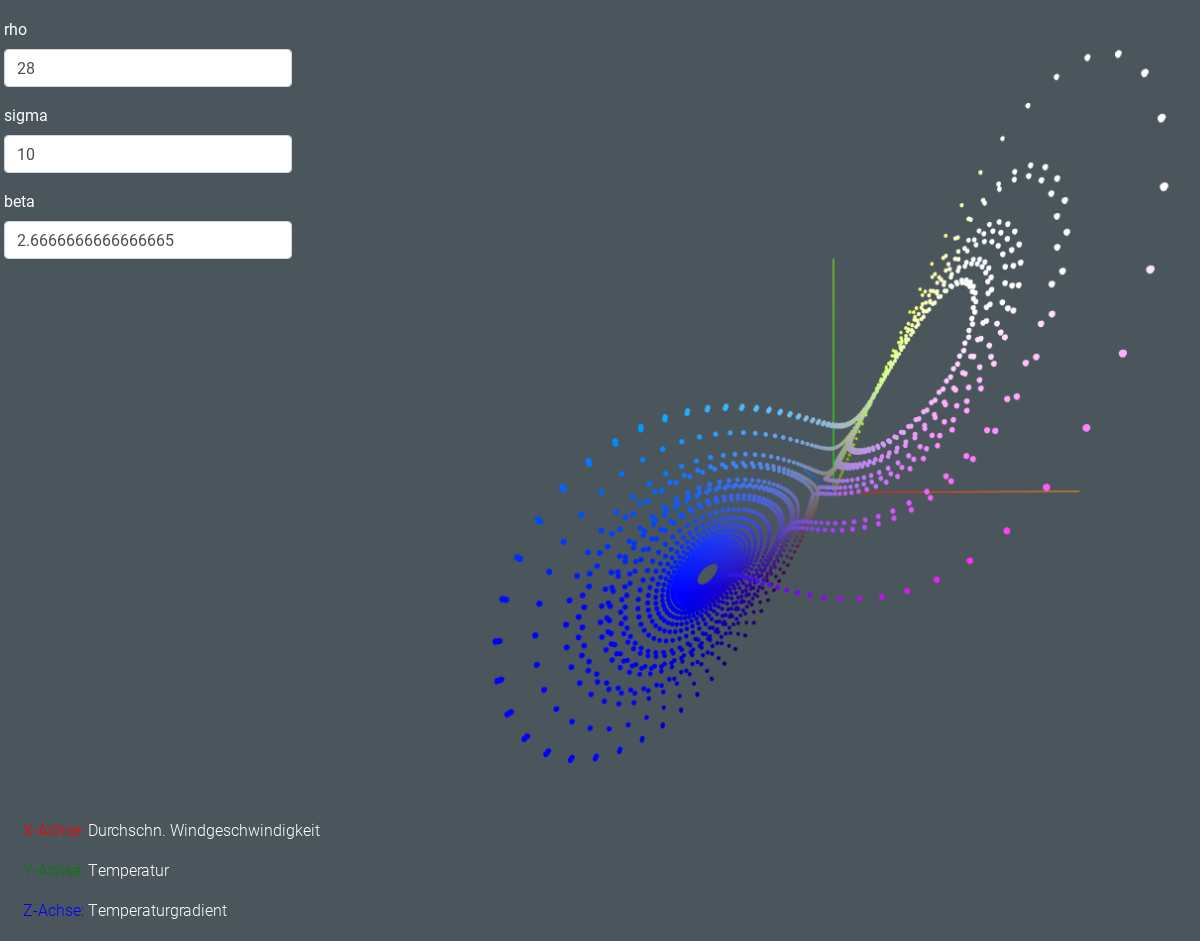
\includegraphics[height=5cm]{lorenz/assets/implementation/Visualisierung}
	\end{centerFigure}
\end{document}
